\section{Image Transform}

\clearpage
\subsection{The discrete cosine transform matrix}

\subsubsection{What does each row of the DCT transform matrix represent? Look at the pattern for each row. If you still don't see it, try plotting each of the rows as a 1-D function.}
Each row of the DCT matrix is a cosine wave, with the period equal to $\frac{\pi}{n} \cdot (i-1)$; where $n$ is the number or rows in the DCT and $i$ is the row of the matrix being examined, with the exception of the first row is constant. The transform of the matrix is given by a product of a cosine oscilating in each direction.

\begin{table}[tbhc]
	\caption{Discrete Cosine Transform Matrix}
	\label{tbl:dctm}
	\begin{center}
		\begin{tabular}{ c | c | c | c | c | c | c | c}
0.3536	&	0.3536	&	0.3536	&	0.3536	&	0.3536	&	0.3536	&	0.3536	&	0.3536	\\
\hline
0.4904	&	0.4157	&	0.2778	&	0.0975	&	-0.0975	&	-0.2778	&	-0.4157	&	-0.4904	\\
\hline
0.4619	&	0.1913	&	-0.1913	&	-0.4619	&	-0.4619	&	-0.1913	&	0.1913	&	0.4619	\\
\hline
0.4157	&	-0.0975	&	-0.4904	&	-0.2778	&	0.2778	&	0.4904	&	0.0975	&	-0.4157	\\
\hline
0.3536	&	-0.3536	&	-0.3536	&	0.3536	&	0.3536	&	-0.3536	&	-0.3536	&	0.3536	\\
\hline
0.2778	&	-0.4904	&	0.0975	&	0.4157	&	-0.4157	&	-0.0975	&	0.4904	&	-0.2778	\\
\hline
0.1913	&	-0.4619	&	0.4619	&	-0.1913	&	-0.1913	&	0.4619	&	-0.4619	&	0.1913	\\
\hline
0.0975	&	-0.2778	&	0.4157	&	-0.4904	&	0.4904	&	-0.4157	&	0.2778	&	-0.0975	\\
		\end{tabular}
	\end{center}
\end{table}


\begin{figure}[ht]
\centering
	\subfigure[Heat map]{
	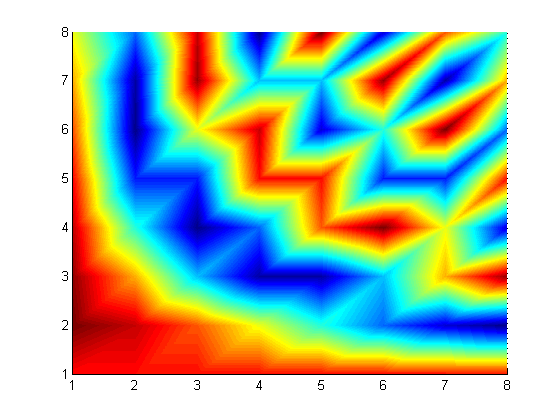
\includegraphics[width=0.45\linewidth]{question3/dctmtx_8_heat}
	}
	\subfigure[Rows of matrix]{
	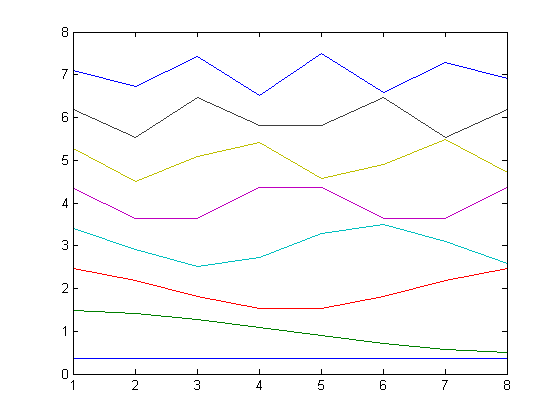
\includegraphics[width=0.45\linewidth]{question3/dctmtx_8_rows}
	}
\end{figure}


\clearpage
\subsection{Applying the discrete cosine transform matrix}



\begin{figure}[ht]
\centering
	\subfigure[Original image]{
	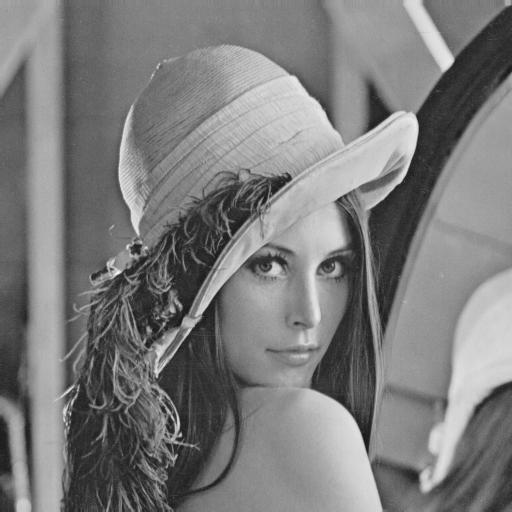
\includegraphics[width=0.45\linewidth]{question3/originalImage}
	}
	\subfigure[DCT 8 $\times$ 8 of original image]{
	
\includegraphics[width=0.45\linewidth]{question3/originalImage_dct}
	}
\end{figure}


\begin{figure}[ht]
\centering
	\subfigure[8 $\times$ 8 image block @ (297,81)]{
	
\includegraphics{question3/block1_8x8}
	}
	\subfigure[DCT]{
		\begin{tabular}{ c c c c c c c c}
		-136 &-31 & 2 &-6 &-1 &-6 &-1 &-4 \\
		14 &-6 & 5 &-6 & 3 &-4 & 2 &-1 \\
		-2 &-3 & 0 &-5 & 3 &-1 & 1 &-2 \\
		1 & 0 & 0 & 2 & 3 &-1 & 0 & 5 \\
		3 & 5 & 0 & 1 & 2 & 4 &-3 & 0 \\
		6 &-1 & 2 & 1 &-1 & 2 & 0 &-1 \\
		0 &-2 & 2 & 0 & 0 &-1 & 0 & 1 \\
		2 &-3 & 0 & 0 &-5 &-3 & 2 & 0 \\
		\\
		\end{tabular}
	}
\end{figure}

\begin{figure}[ht]
	\centering

	\subfigure[8 $\times$ 8 image block @ (1,1)]{
	
\includegraphics{question3/block2_8x8}
	}
	\subfigure[DCT]{
		\begin{tabular}{ c c c c c c c c}
		259 & 4 & 3 &-1 & 0 &-1 &-5 & 5 \\
		7 &-1 & 0 &-5 & 1 & 2 &-4 & 3 \\
		-6 &-1 &-2 & 1 &-1 &-1 & 1 &-3 \\
		2 & 1 & 1 & 0 &-1 &-2 & 0 & 1 \\
		-1 &-2 &-1 &-2 & 1 & 1 &-2 &-1 \\
		1 & 0 &-2 &-1 &-3 & 0 & 1 & 0 \\
		-2 & 0 & 3 & 1 & 1 &-3 &-2 &-1 \\
		1 &-1 &-3 &-2 &-1 & 1 & 0 & 0 \\
		\\
		\end{tabular}
	}
\end{figure}


\subsubsection{Describe the energy distribution of the DCT of the sub-images. What does each pixel represent? Explain why DCT would be useful for image compression in the context of the DCT energy distribution}

\subsubsection{Compare the DCT of the two sub-images. How are they different? Why? Explain in the context of the image characteristics at those locations and the DCT energy distribution}

\subsection{Compressing the DCT image by discarding high-frequency data}

\subsubsection{Describe how the reconstructed image looks compared to the original image. Why does it look this way?}

\subsubsection{What artifact is most prominent in the image? Why does this artifact appear?}

\subsubsection{What conclusions can you draw about the DCT in terms of image compression? Does it work well? If yes, why does it work well?}